\documentclass{article}
\usepackage[dblblindworkshop]{neurips_2026}
\usepackage{amsmath,amssymb,booktabs,graphicx,microtype,xcolor}
\usepackage{hyperref}
\usepackage{enumitem}
\newcommand{\dev}{\textsc{development-only}}
\newcommand{\obs}{\textsc{observational}}
\newcommand{\TODO}[1]{\textcolor{red}{[TODO: #1]}}
\title{When Evaluation Cues Become the Evaluation: Auditing Purpose-by-Format Probes in Language Models}
\author{Anonymous Workshop Submission}
\workshoptitle{TAE (Trust-AI-Eval): Can We Trust AI Evaluation?}

\begin{document}
\maketitle

\begin{abstract}
Evaluation protocols can produce highly reproducible internal signals without measuring the construct that their interpretation invokes. We study this failure mode in a frozen purpose-by-format evaluation design. Each payload is crossed between an evaluation and deployment purpose and between benchmark and casual response formats, allowing purpose effects, format offsets, and purpose--format interactions to be estimated separately. On 11,520 rendered items from 320 payload blocks, held-out cue-vocabulary probes decode stated response purpose strongly across Llama-3.1-8B, Llama-3.1-70B, and Llama-3.3-70B. However, format is also highly decodable, threshold accuracy can remain near chance when AUC is high, and a direct 8B Jacobian-lens diagnostic yields much weaker purpose readouts than the conventional probe. An equal-training-size control at 8B preserves purpose decodability, but does not establish a behavioral or causal endpoint. The resulting evidence supports a methodological conclusion: decodability of evaluation-context cues is not evidence of evaluation awareness. We provide the frozen data contract, model revisions, activation hashes, control analyses, and explicit claim boundaries needed to audit this class of evaluation protocol.
\end{abstract}

\section{Introduction}
Benchmarks frequently attach high-level interpretations to low-level measurements. A model that responds differently when told that an answer will be judged may be described as exhibiting evaluation awareness, strategic behavior, or situational reasoning. Each description requires more than a classifier that separates two prompt conditions. It requires a validated construct, a protocol that isolates the construct from formatting and sampling artifacts, and an endpoint connecting the internal signal to behavior or a decision.

This paper audits a purpose-by-format evaluation protocol rather than treating its strongest probe score as a discovery. The protocol crosses two factors: stated response purpose (evaluation versus deployment) and response format (benchmark versus casual). The crossing makes it possible to distinguish a format-shared purpose effect from a format offset and an interaction. It also creates direct failure tests: if a purpose signal disappears under format transfer, or if fixed-threshold accuracy disagrees with AUC, the protocol does not support a simple interpretation.

Our main result is deliberately narrower than an awareness claim. On a frozen 320-block dataset, purpose is strongly decodable using held-out cue-vocabulary splits in three Llama models. Yet the same representation carries strong format/template information, and a direct 8B Jacobian-lens diagnostic is substantially weaker for purpose than the conventional probe. The appropriate conclusion is that the protocol measures a reproducible stated-purpose signal, while the intended latent construct remains underdetermined.

Our contributions are: (1) a hash-anchored full320-v3 evaluation freeze with a crossed purpose--format design; (2) matched observational probes that report AUC and balanced accuracy separately; (3) cue-excision, transfer, and equal-training-size controls; (4) a model-specific 8B direct-lens diagnostic; and (5) a claim-audit framework that distinguishes decodability, geometry, internal mediation, behavioral causality, and confirmation.

\section{Target construct and protocol}
\subsection{What is measured}
We use \emph{stated response purpose decodability} as the primary estimand. A rendered prompt states that a response will be evaluated or deployed, and the model's last-prompt-token residual representation is probed for that label. We do not equate this estimand with evaluation awareness. In particular, a probe may recover lexical, stylistic, calibration, or task-format information correlated with the purpose statement.

The frozen full320-v3 data contain 11,520 rendered items from 320 payload blocks. Each block is crossed over purpose $p\in\{E,D\}$ and format $f\in\{B,C\}$, where $E/D$ denote evaluation/deployment and $B/C$ denote benchmark/casual format. The intended effect-coded decomposition is
\begin{equation}
 h_{p,f}=\mu+pA+fB+pfC+\epsilon,
\end{equation}
where $A$ is the format-shared purpose effect, $B$ is the format offset, and $C$ is the purpose--format interaction. The primary dataset hash is
\texttt{5528819d74e696d1a595062047a829836dfde1d2a45287b06a5ac1ba5d1b6c67}.

\subsection{Activation contract}
For each model, activations are the zero-based transformer-block output before final model normalization at the last prompt token after applying the user-only chat template with generation prompt. Inference uses BF16 and saved activations are FP32. The pinned model revisions are Llama-3.1-8B-Instruct (\texttt{0e9e39f2}), Llama-3.1-70B-Instruct (\texttt{1605565b}), and Llama-3.3-70B-Instruct (\texttt{6f6073b4}). The complete per-file provenance is recorded in the accompanying HF snapshot and evidence manifest.

\subsection{Held-out evaluation}
The conventional probe is StandardScaler followed by logistic regression with $C=0.1$, maximum 3000 iterations, and fixed random state 0. We use five held-out cue-vocabulary folds. The principal regime trains on all four purpose--format cells and tests within the held-out vocabulary fold. We also report benchmark-to-casual and casual-to-benchmark transfer. AUC and balanced accuracy are separate endpoints: AUC is threshold-free, while balanced accuracy uses the fitted decision threshold and can expose calibration failure.

\section{Full320 observational results}
Table~\ref{tab:peaks} reports each model's peak decorrelated layer from the pinned result files. Peak selection is descriptive for this table; the full trajectories are included in the supplement and are not treated as independent replications across layers.

\begin{table}[t]
\caption{Pinned full320 observational results at the decorrelated AUC peak.}
\label{tab:peaks}
\centering
\begin{tabular}{lrrrrr}
\toprule
Model & Layer & Purpose AUC & Purpose BA & B$\rightarrow$C AUC & C$\rightarrow$B AUC\\
\midrule
Llama-3.1-8B & 8 & .9888 & .9409 & .9513 & .9401\\
Llama-3.1-70B & 18 & .9984 & .9788 & .9846 & .9850\\
Llama-3.3-70B & 18 & .9959 & .9659 & .9845 & .9787\\
\bottomrule
\end{tabular}
\end{table}

Purpose decodability is therefore reproducible under held-out cue vocabulary and remains high under cross-format transfer. This is evidence for a stable signal in the protocol. It is not evidence that the signal is a uniquely semantic representation of evaluation status. The confounded regime illustrates why endpoint choice matters: its AUC can exceed .60 while balanced accuracy remains close to chance at the model peaks. A score that ranks examples well but fails at its operating threshold is not interchangeable with a reliable decision rule.

\begin{figure}[t]
\centering
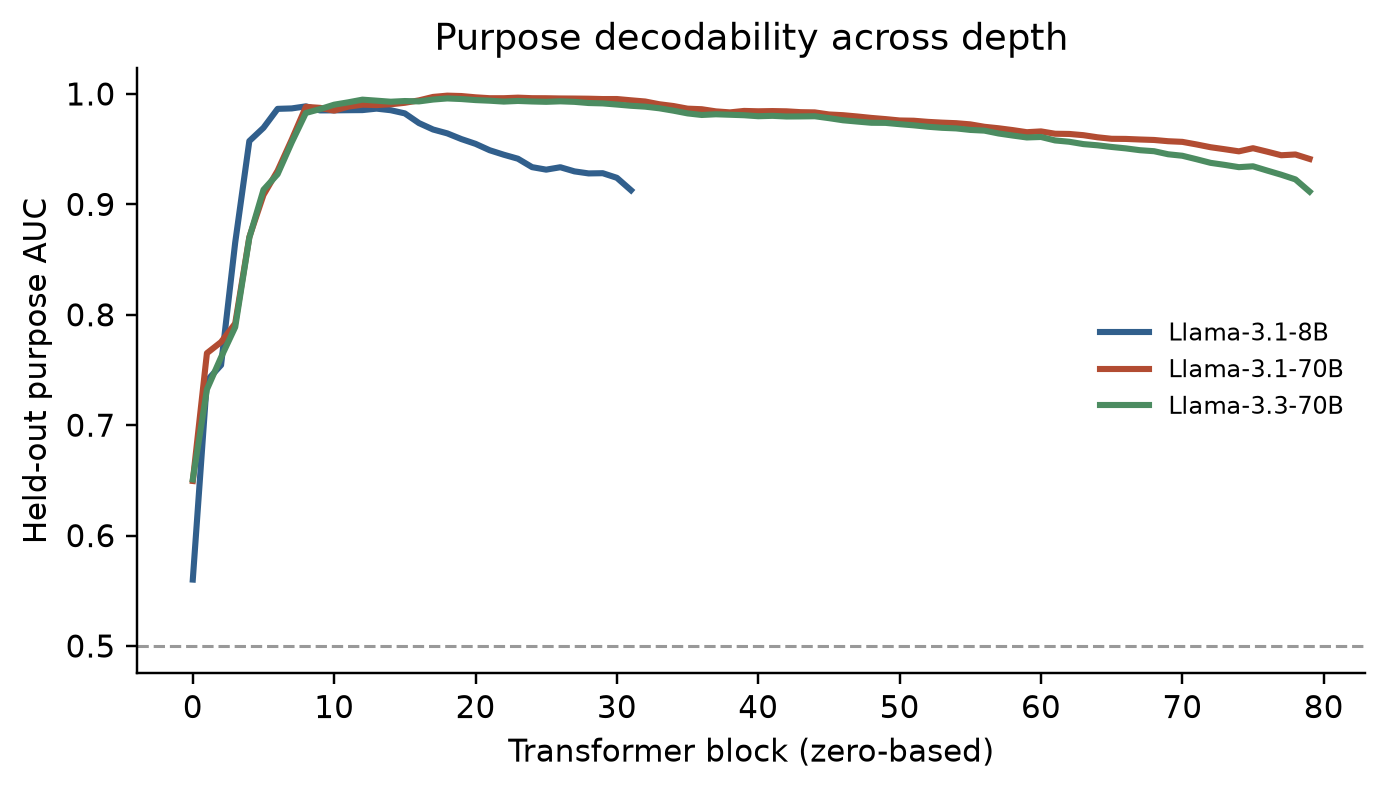
\includegraphics[width=.92\linewidth]{figures/main_purpose_by_depth.png}
\caption{Held-out purpose AUC across all layers using the pinned full320 result arrays. The figure is \obs and does not establish a causal or awareness construct.}
\label{fig:depth}
\end{figure}

\begin{figure}[t]
\centering
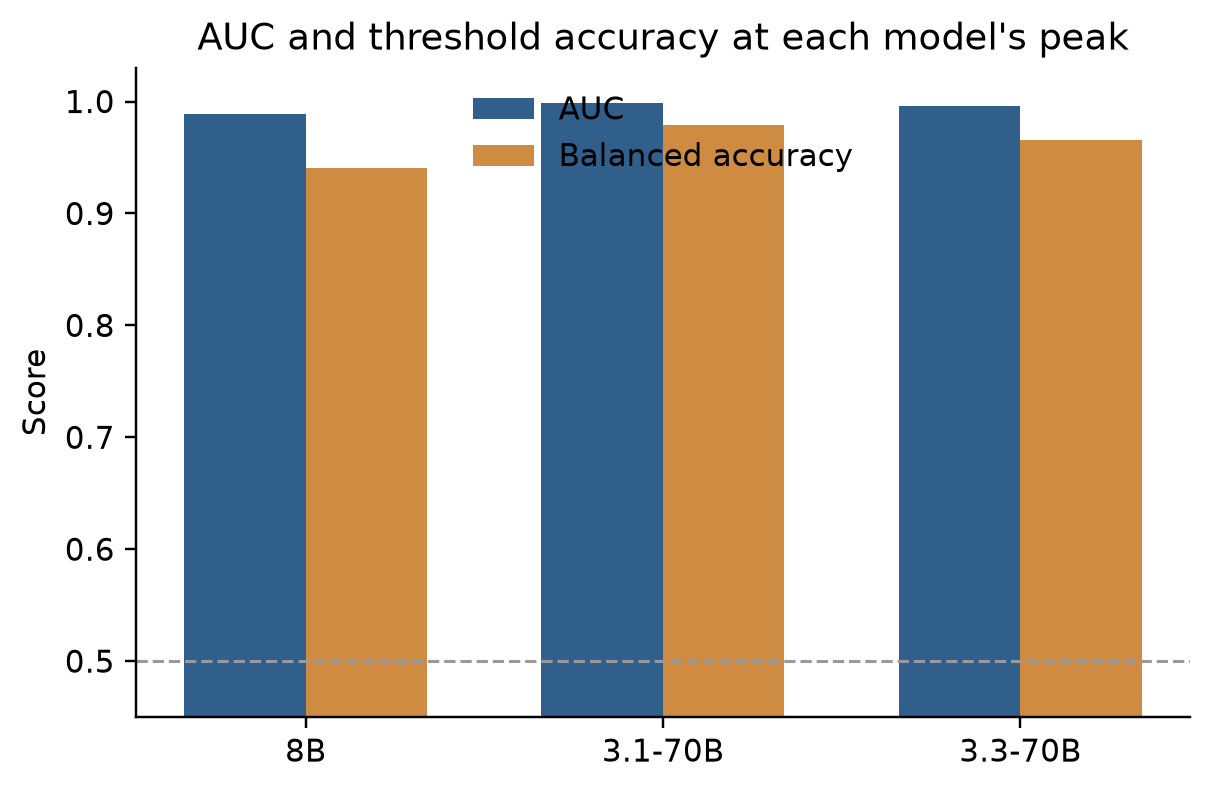
\includegraphics[width=.92\linewidth]{figures/main_auc_balanced_accuracy.png}
\caption{AUC and balanced accuracy at each model's descriptive peak. Keeping these endpoints separate exposes calibration differences.}
\label{fig:calibration}
\end{figure}

\begin{figure}[t]
\centering
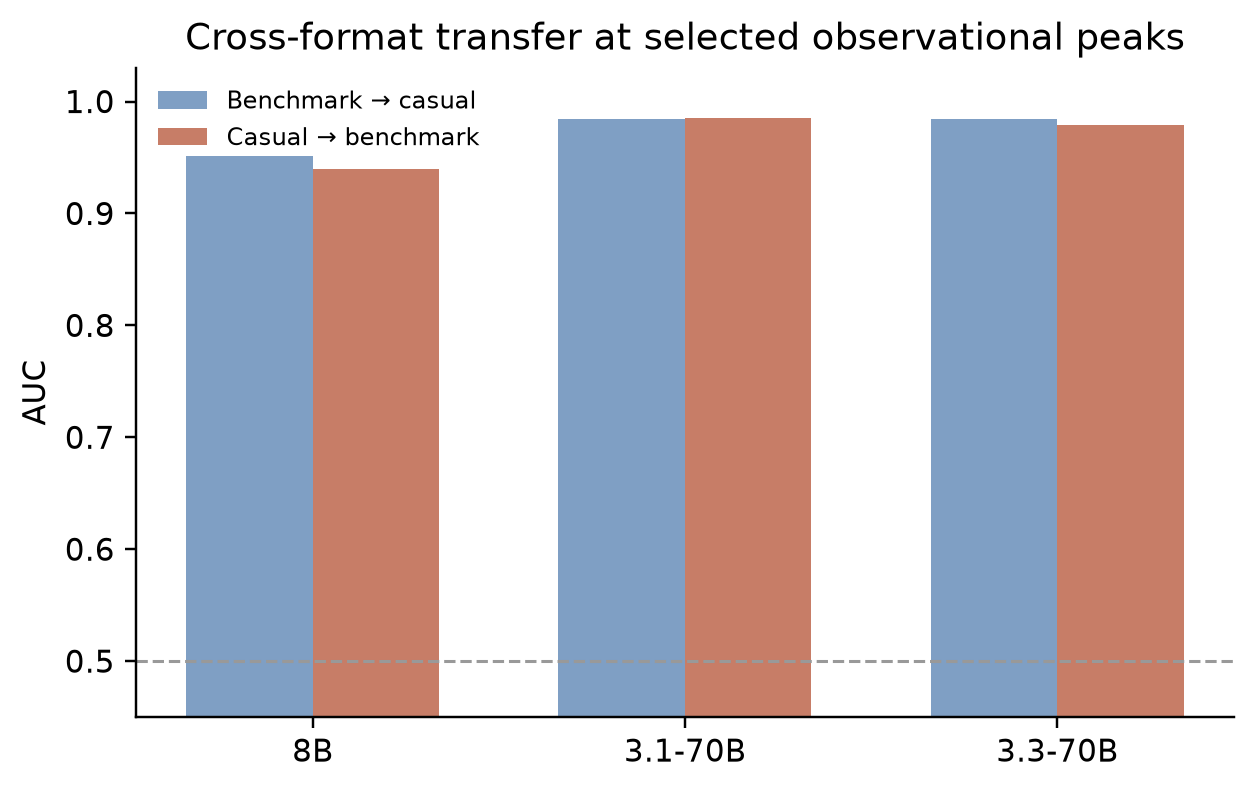
\includegraphics[width=.92\linewidth]{figures/main_cross_format_transfer.png}
\caption{Cross-format transfer at each model's descriptive observational peak. Transfer is a protocol property, not evidence of a causal awareness variable.}
\label{fig:transfer}
\end{figure}

\section{Protocol audits}
\subsection{Surface and format controls}
The cue-excision surface battery removes the intended purpose words and reports near-chance purpose AUC for its four purpose controls. This is a useful negative control for direct lexical copying. It does not remove every possible surface or task-structure feature: format, template identity, and contract identity remain intentionally decodable. In the full320 surface audit, format AUC is approximately .798, template-ID accuracy is approximately .908, and contract accuracy is approximately .983. These values show that the protocol contains designed structure beyond the purpose label.

\subsection{Equal-training-size control}
The raw cross-format comparison can be confounded by training-row count. We therefore implemented a fixed-seed equal-training-size mixed-format control at 8B layer 12. For each held-out purpose-family fold, benchmark-only, casual-only, and mixed-format regimes use the same number of training payload blocks; the mixed regime balances format assignments over blocks. Complete payload blocks are the bootstrap unit.

\begin{table}[t]
\caption{8B equal-training-size control at layer 12. Values are means over four fixed seeds; confidence limits are means of the 1,000 block-bootstrap limits.}
\label{tab:equaln}
\centering
\begin{tabular}{lrrrr}
\toprule
Training regime & AUC & BA & AUC 2.5\% & AUC 97.5\%\\
\midrule
Benchmark-only & .9588 & .8949 & .9553 & .9625\\
Casual-only & .9538 & .8775 & .9502 & .9575\\
Equal-N mixed & .9797 & .9241 & .9773 & .9821\\
\bottomrule
\end{tabular}
\end{table}

This control removes one important alternative explanation for the 8B result: an unequal number of training rows alone is not required for high held-out purpose decodability. It does not validate the construct, and it has not yet been run for the two 70B models. Accordingly, we make no all-model equal-N claim.

\begin{figure}[t]
\centering
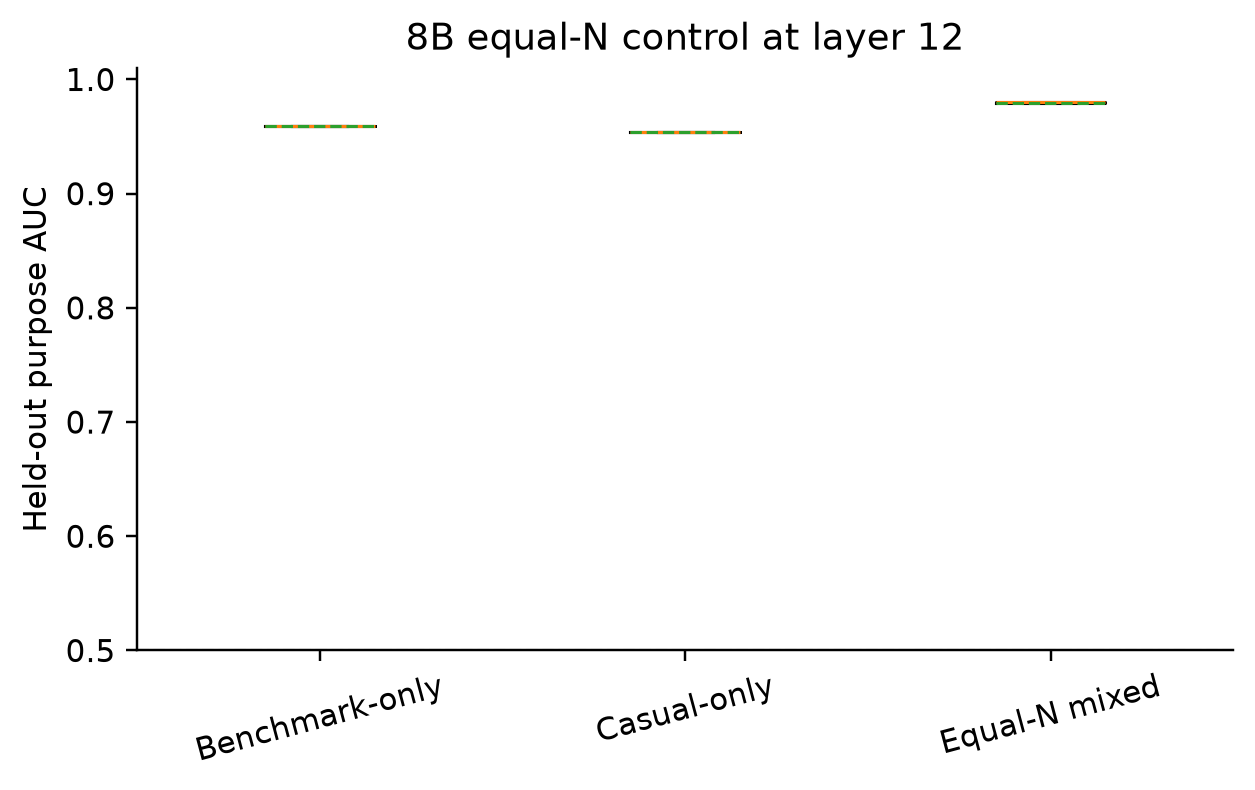
\includegraphics[width=.92\linewidth]{figures/main_equal_n_8b.png}
\caption{8B equal-training-size control. This is a development control for one model and one predeclared layer, not a confirmation result.}
\label{fig:equaln}
\end{figure}

\section{Direct mechanistic diagnostic}
We fit a model-specific Jacobian lens on 1,000 generic FineWeb prompts for Llama-3.1-8B and apply it to the full320 rows. The lens is FP32, uses source layers 4, 9, 12, 15, 20, and 24, and targets layer 31. The assay is explicitly \dev: it scores scalar concept-logit differences for evaluation/deployment concept groups and a no-cue format diagnostic.

The oriented purpose AUC across source layers 4, 9, 12, 15, 20, and 24 is approximately .513, .569, .612, .577, .608, and .576. The corresponding no-cue format AUC reaches approximately .622, .570, .622, .671, .534, and .559. Thus the direct purpose readout is much weaker than the conventional held-out probe, while format remains visible. A scalar factorial bootstrap over 320 blocks gives positive $A$ at several later source layers but small $C$ relative to $A$; $C/|A|$ intervals are unstable and often overlap zero.

\begin{figure}[t]
\centering
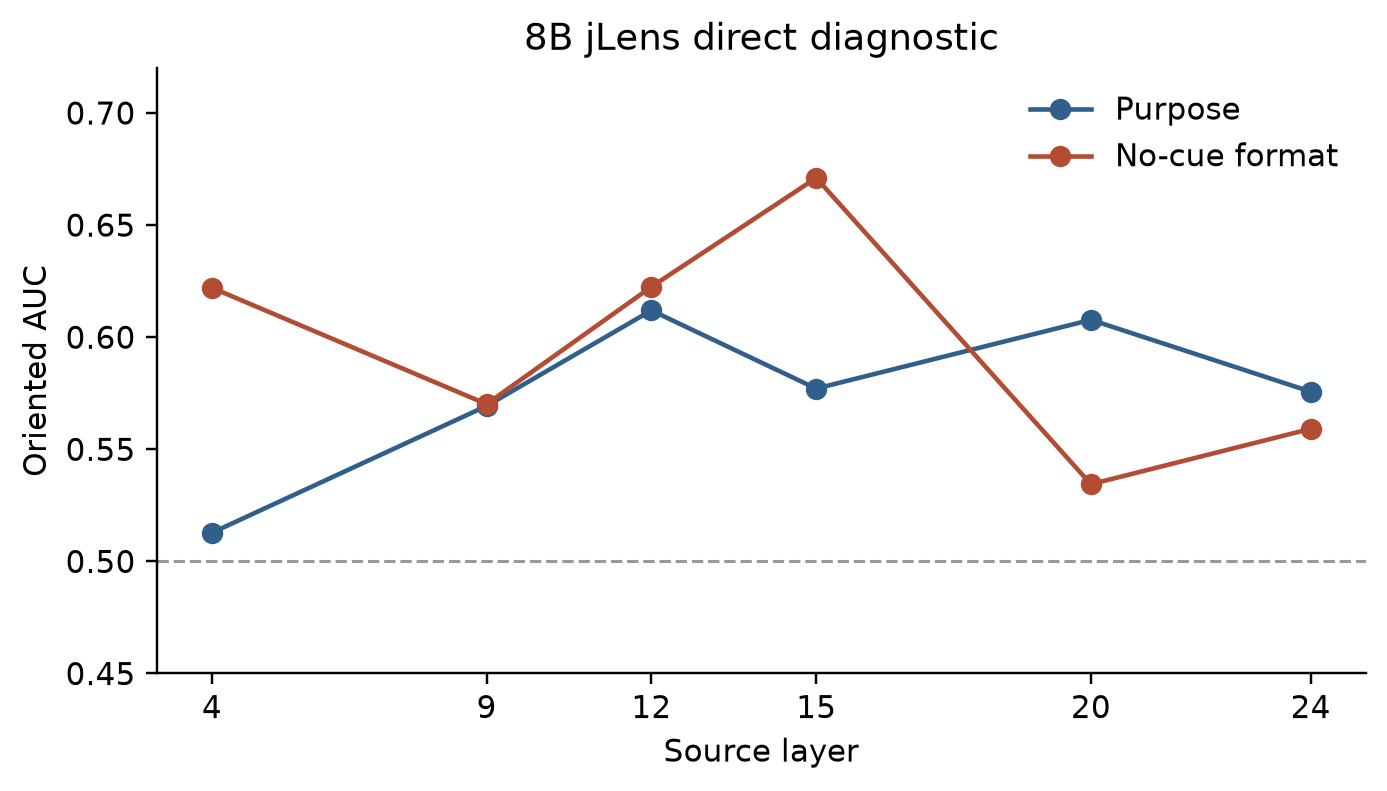
\includegraphics[width=.92\linewidth]{figures/appendix_jlens_direct_diagnostic.png}
\caption{Direct 8B Jacobian-lens diagnostic. Purpose and no-cue format readouts are both \dev; neither is a behavioral endpoint.}
\label{fig:jlens}
\end{figure}

This result does not falsify all internal mediation hypotheses. It does show that the conventional probe result and the direct lens result are not interchangeable. We therefore report the lens as a mechanistic diagnostic, not as evidence of spontaneous evaluation awareness or behavioral steering.

\section{What the protocol supports}
The evidence supports four bounded conclusions. First, stated response purpose is decodable from the frozen model representations under held-out cue-vocabulary evaluation. Second, the signal transfers across the two response formats in the conventional probe. Third, format and template structure are independently visible and threshold calibration matters. Fourth, a direct 8B lens diagnostic does not reproduce the strength of the conventional purpose probe.

The evidence does not support a claim that models possess a latent evaluation-awareness variable, that a purpose direction causally changes behavior, or that the effect scales to Llama-3.1-405B. No 405B activation bundle or model revision is available in the frozen evidence package. The independent devbunova 2x2 dataset has no matched local activations and is used only as provenance/context in the appendix. The pilot80-v2 data are a separate exploratory freeze and are not pooled with full320.

\section{Limitations and reporting checklist}
The primary limitation is construct validity: a linear probe can recover information correlated with a prompt manipulation without identifying the intended psychological or computational construct. The equal-N control is currently 8B-only. The direct lens is also 8B-only, scalar, and development-only. We do not have an independent validated behavioral endpoint whose unsteered accuracy and calibration would justify causal intervention. Layers are repeated measurements within a model, not independent samples. Finally, the local regenerated result arrays differ bytewise from the pinned HF result files; all reported full320 numbers in this paper use the pinned result copies and their recorded revision/hash chain.

Our reporting checklist is therefore: define the construct before inspecting outcomes; report the complete layer trajectory; separate AUC from threshold accuracy; preserve the purpose--format factorial decomposition; use payload blocks as the uncertainty unit; report equal-N status; distinguish observational probes, geometry, internal mediation, and behavioral causality; and publish item, activation, model, code, and output hashes.

\section{Conclusion}
An evaluation protocol can be highly reproducible and still be insufficient for the claim attached to it. The full320 audit demonstrates strong stated-purpose decodability, but also exposes format structure, calibration failures, and a weaker direct mechanistic diagnostic. The practical lesson is not that evaluation-context probes are useless. It is that their outputs must be treated as measurements requiring construct, sampling, calibration, and causal validation—not as awareness detectors by default.

\appendix
\section{Reproducibility inventory}
The canonical dataset is pinned at \texttt{format-EA/full320-v3} revision \texttt{d6c3be7be83c469d9a6a2aa4e797f3a7d...} and contains 11,520 rows from 320 payload blocks. Full activation and result hashes are recorded in \texttt{provenance/full320-v3/hf\_snapshot.json}. The submission evidence inventory is \texttt{artifacts/submission\_sprint\_manifest.json}; the figure inventory is \texttt{artifacts/submission\_figure\_manifest.json}. The equal-N output is \texttt{artifacts/full320\_equal\_n\_llama31\_8b\_l12.json}. All current outputs are marked \dev.

\section{Additional pilot and dataset context}
The pilot80-v2 activation freeze contains 1,760 rows and is anchored by item hash \texttt{0dbcb9802924d3c2063fce87e24250d1a3430fd24856ea83b132e606843f6638}. It is reported separately as exploratory context. The devbunova parquet files are independent data with different identifiers and schemas; because no matched activations are present, they are not used as a robustness replication.

\end{document}
